% Budget: ~1.25 columns  |  10 pts.  Slides p.9.
% Sources: EDA/README.md and EDA/tables/feature_ranking.csv (P2), results/README.md (I2).
% Figure 1 is an English re-plot of P2's figure from data/outputs/p1/train_readable.csv
%   (same r and rho); script: figures/plot_qualityarea.py
\section{Exploratory Feature Analysis}
\label{sec:eda}

\textbf{Association.} Using only the 1{,}166 training sales and $\log(1+\text{price})$ as the target, we rank 32 numeric features by Pearson and Spearman correlation, and all 73 candidate features by mutual information (MI).
Overall quality leads on all three measures (Pearson $r = 0.813$, Spearman $\rho = 0.803$, MI $= 0.544$ nats), followed by living area ($r = 0.719$).
Neighborhood ranks second by MI (0.495), an importance of location that only MI can reveal for a categorical feature.
Construction year and garage size complete the top group.

\textbf{Redundancy.} Three pairs exceed $|r| = 0.8$: garage cars and garage area (0.889), living area and total rooms (0.826), and basement and first-floor area (0.808).
After one-hot encoding, the design matrix is rank-deficient by 22.6 columns on average across folds.
This collinearity argues against plain OLS (\S\ref{sec:method}).

\textbf{Hypotheses.} The evidence suggests three feature designs, each tested in \S\ref{sec:results}:
\begin{itemize}
  \item \textbf{H1 (interaction).} The product QualityArea $=$ OverallQual $\times$ GrLivArea correlates more strongly with price ($r = 0.836$, $\rho = 0.850$; Figure~\ref{fig:eda}) than either factor alone. Extra space may be worth more in a better-built house.
  \item \textbf{H2 (log transform).} Taking $\log(1+\text{LotArea})$ raises $r$ from 0.261 to 0.415, suggesting diminishing returns to lot size.
  \item \textbf{H3 (aggregation).} Total area TotalSF (basement $+$ first $+$ second floor) has $r = 0.822$ and could replace three correlated columns without losing accuracy.
\end{itemize}
Correlation is not predictive gain, so each hypothesis is kept only if it lowers cross-validated error.

\begin{figure}[t]
\centering
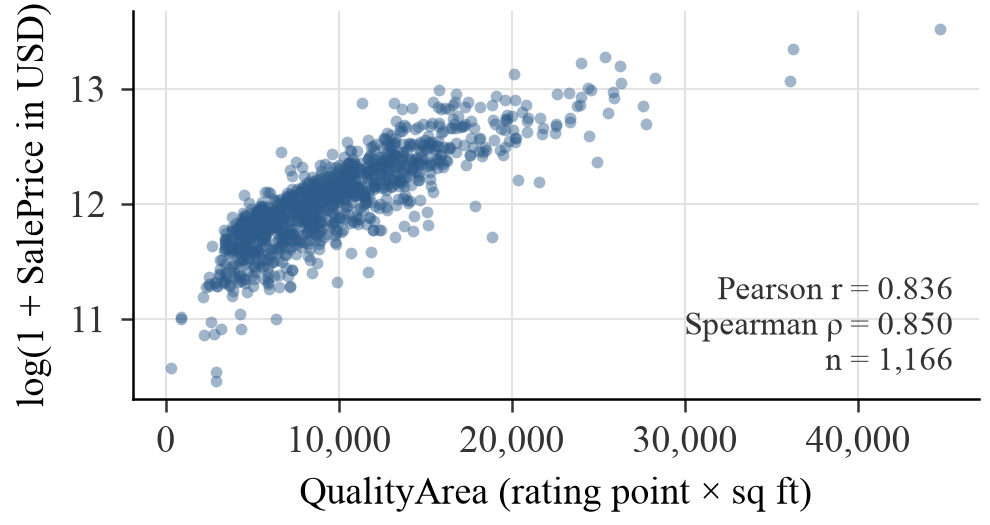
\includegraphics[width=\columnwidth]{figures/eda_qualityarea.png}
\caption{QualityArea (OverallQual $\times$ GrLivArea) against log sale price on the training data ($n = 1{,}166$), the evidence behind H1; its predictive gain is tested in \S\ref{sec:results}.}
\label{fig:eda}
\end{figure}
